\documentclass{protokol}
\usepackage[T1]{fontenc}
\leftheader{Studium plynových detektorů}
\centerheader{Praktikum IV}
\rightheader{Tomáš Derner}

\begin{document}

    \section*{Úkol}

    \begin{enumerate}
        \item Pomocí ionizační komory (IK) zjistěte, který z přiložených radioaktivních zářičů má větší aktivitu.

        \item Změřte V-A charakteristiky IK v rozsahu $0-\SI{500}{V}$ při různých vzdálenostech elektrod $1-\SI{6}{cm}$.
        Použijte intenzivnější zářič.

        \item Identifikujte charakteristické oblasti V-A závislostí.
        Určete optimální napětí a optimální vzdálenost elektrod IK.

        \item Změřte závislost svodového proudu na napětí v rozsahu $0-\SI{500}{V}$ při optimální vzdálenos\-ti elektrod.

        \item Změřte poměr aktivit přiložených zářičů, odhadněte jejich absolutní aktivity (střední energie na vytvoření iontového páru ve vzduchu je $\SI{35}{eV}$).
        Stanovte dosah $\alpha$-částic ve vzduchu.

        \item Pomocí osciloskopu změřte závislost amplitudy elektrického impulzu Geiger-Müllerova (GM) detektoru na napětí v rozsahu $0-\SI{1500}{V}$.
        Nepřekračujte napětí $\SI{1500}{V}$ aby nedošlo k destrukci GM detektoru!
        \item Identifikujte charakteristické oblasti V-A závislosti GM detektoru.

    \end{enumerate}

    \section*{Teorie}

    Cílem měření bylo zkoumání vlastností ionizační komory a Geiger-Müllerova detektoru.
    Využí\-váme přitom zdroje záření $\alpha$.

    Ionizační komora je realizována jako deskový kondenzátor.
    Proud $\alpha$ částic ionizuje vzduch a tudíž zvyšuje počet volných nositelů proudu.
    Do určitého napětí na deskách kondenzátoru splňuje ionizační proud ohmův zákon, po dosažení kritického napětí již proud na zvyšujícím se napětí nezávisí, protože všechny nosiče proudu získané ionizací jsou uneseny k elektrodám dříve, než stačí rekombinovat, toto je oblast nasyceného proudu.
    Tato poloha je pro činnost ionizační komory nejvhodnější.
    Ionizační komora umožňuje určit energie a typy částic způsobujících ionizaci.
    Úplná voltampérová charakteristika plynových detektorů je zobrazena na obrázku~\ref{fig:regions} a detailní popis charakteristických úseků lze nalézt v~\cite{pokyny}.

    \begin{figure}[h]
        \centering
        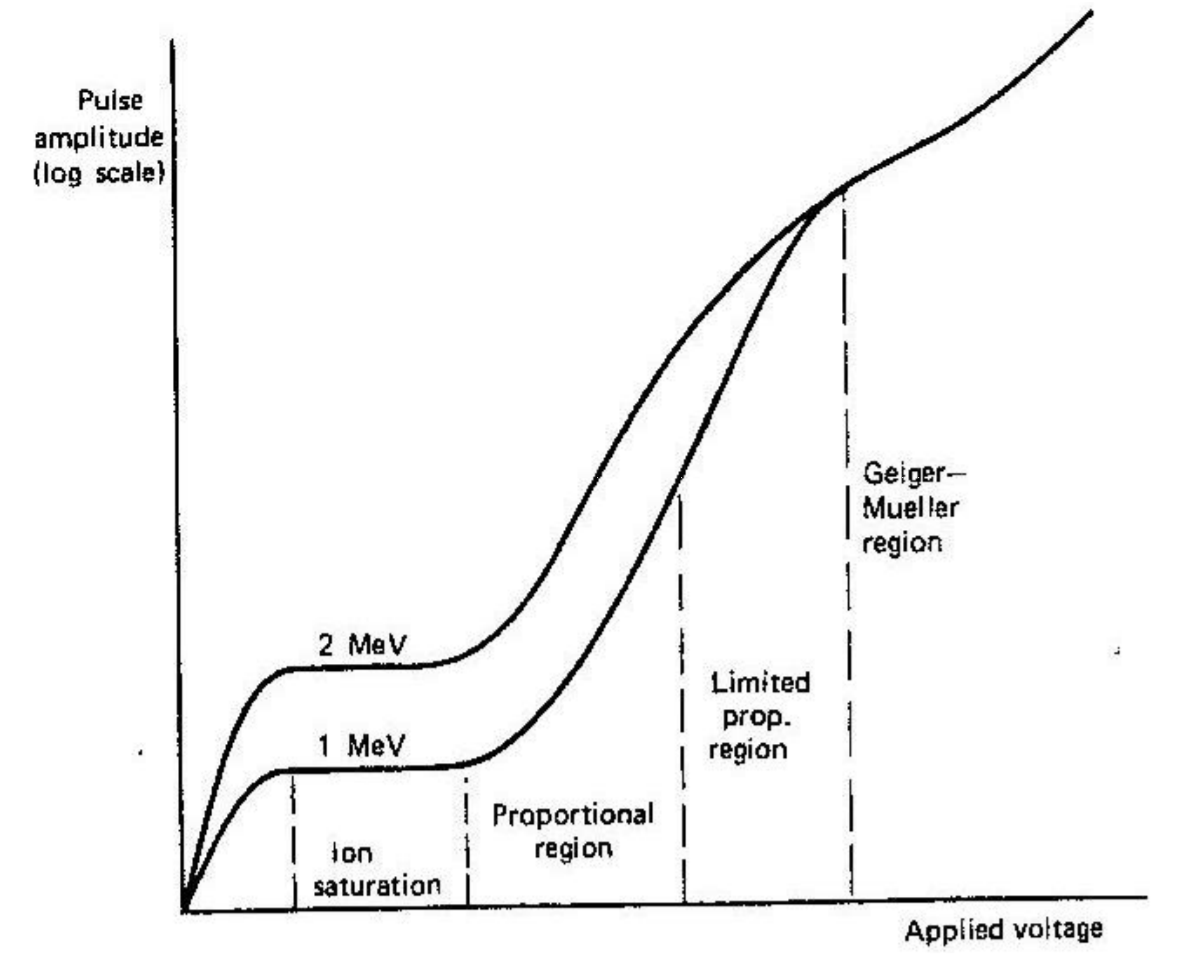
\includegraphics[height=220pt]{regions.png}
        \caption{Voltampérová charakteristika plynových detektorů, převzato z~\cite{pokyny}}
        \label{fig:regions}
    \end{figure}

    Průběh závislosti ionizačního proudu na přiloženém napětí také samozřejmě závisí na vzdálenosti desek kondenzátoru $d$.
    Je výhodnější pracovat s větší vzdáleností desek, protože vzniká více nositelů náboje ionizací.
    Částice $\alpha$ mají však dráhu doletu jen několik centimetrů, nemá proto velký smysl nastavovat vzdálenost $d$ větší, než je právě vzdálenost doletu.

    $\alpha$ částice, se kterými v praktiku pracujeme, mají kinetickou energii $E_\alpha \approx \SI{8.776}{MeV}$.
    Předpokládáme-li, že částice ztratí veškerou kinetickou energii v komoře, můžeme odhadnout aktivitu zářiče
    \begin{equation}
        \label{eq:A}
        A = \frac{I}{e} \frac{E_i}{E_\alpha},
    \end{equation}
    kde $I$ je proud tekoucí komorou v oblasti nasycení, $e$ je elementární náboj a $E_i = 35 eV$ je ionizační energie vzduchu.

    Při měření je také použit Geiger-Müllerův detektor, sestávající z trubice vyplněné netečným plynem a elektrody uvnitř této trubice.
    Na trubici a elektrodu je přiloženo vysoké napětí.
    Při ionizaci plynu prolétající částicí vzniká detekovatelný puls v napětí a proudu mezi trubicí a elektrodou.
    Geiger-Müllerův detektor pracuje v Geiger-Müllerově oblasti, proto nejsou tyto detektory schopny rozlišit energie částic a tedy ani jejich povahu.

    \section*{Výsledky}

    Do ionizační komory byly po sobě vloženy dva zdroje $\alpha$ záření EA13 a EA14.
    Při vzdálenosti $d=\SI{6}{cm}$ a napětí $U = \SI{500}{V}$ byly změřeny ionizační proudy

    \[I_{EA13} = \SI{0.8 \pm 0.2}{pA},\]
    \[I_{EA14} = \SI{12.7 \pm 0.5}{pA}.\]

    Z výsledků je zřejmé, že silnějším zdrojem záření je zdroj EA14.

    Pro vzdálenosti $d = 2$ a $ \SI{6}{cm}$ byly proměřeny voltampérové charakteristiky ionizační komory v rozsahu napětí $0 - \SI{500}{V}$ za použití zářiče EA14.
    Naměřené závislosti jsou zaznamenány v tabulce~\ref{tab:u2} a grafu na obrázku ~\ref{fig:u2}.

    \begin{table}[h]
        \centering
        \setlength{\tabcolsep}{15pt}
        \begin{tabular}[t]{
  S[table-format=1.3]
  S[table-format=3.1]
  S[table-format=1.1]
} \toprule
{$I_{mag}$} & {$U_{kr}$} & {$\sigma_{U_{kr}}$} \\
{[A]}       & {[V]}      & {[V]}               \\ \midrule
      0.508 &        8.4 &                 0.5 \\
      0.758 &       19.4 &                 0.8 \\
      0.996 &       32.8 &                 1.0 \\
      1.202 &       47.0 &                 0.7 \\
      1.405 &       64.0 &                 0.7 \\
      1.602 &       82.6 &                 0.7 \\
      1.701 &       92.4 &                 0.8 \\
      1.791 &      101.8 &                 0.7 \\
      1.889 &      112.0 &                 1.0 \\
      2.010 &      124.3 &                 1.1 \\ \bottomrule
\end{tabular}
        \caption{Voltampérová charakteristika ionizační komory pro dvě vzdálenosti $d$}
        \label{tab:u2}
    \end{table}

    \begin{figure}[h!]
        \centering
        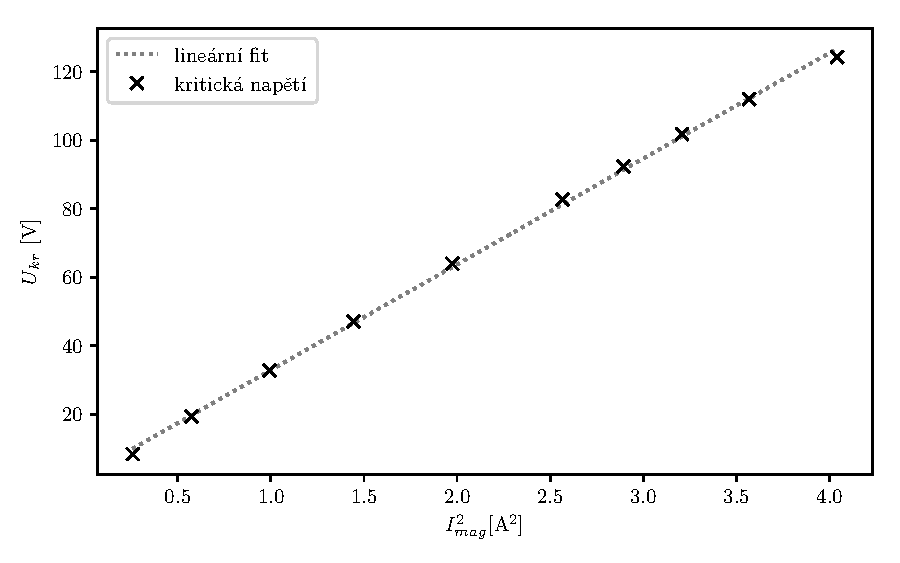
\includegraphics{u2.pdf}
        \caption{Voltampérová charakteristika ionizační komory pro dvě vzdálenosti $d$}
        \label{fig:u2}
    \end{figure}

    Je zřejmé, že první část grafu, kde proud prudce roste s napětím, je oblast Ohmova zákona, druhá část oblast nasyceného proudu.
    Z teorie vyplývá, že optimální napětí je v oblasti nasyceného proudu, je proto výhodné měřit s napětím $U = \SI{500}{V}$, a že je vhodnější použít větší vzdálenost elektrod, proto volíme $d = \SI{6}{cm}$.

    Následně byl změřen svodový proud, tj. proud bez přítomnosti zdroje záření, pro $U = \SI{500}{V}$ a optimální vzdálenost elektrod $d = \SI{6}{cm}$:
    \[ I_{svod} = \SI{0.1 \pm 0.2}{pA},\]
    což je hodnota v rámci chyby shodná s nulou.
    Proto bylo upuštěno od měření celé charakteristiky.

    Pomocí vztahu~\eqref{eq:A} vypočítáme aktivitu zářiče EA13 a EA14
    \[ A_{EA13} = \SI{20}{Bq}, \]
    \[ A_{EA14} = \SI{316}{Bq}. \]
    Skutečné hodnoty aktivit (napsané v praktiku na krabičkách se zářiči) jsou $A_{EA13} = \SI{99.5}{Bq}$, $A_{EA14} = \SI{1485}{Bq}$.

    Pomocí osciloskopu byla změřena závislost amplitudy elektrického impulzu Geiger-Müllerova detektoru na napětí v rozsahu $900-\SI{1500}{V}$.
    Pro nižší hodnoty napětí nebyla pozorována odezva.
    Výsledky jsou uvedeny v tabulce~\ref{tab:u6} a zobrazeny v grafu na obrázku~\ref{fig:u6}.
    Závislost je exponenciální a nevykazuje výrazné změny, lze tedy usoudit, že se detektor po celou dobu měření nacházel v Geiger-Müllerově oblasti.

    \begin{table}[h]
        \centering
        \setlength{\tabcolsep}{15pt}
        \begin{tabular}[t]{
S[table-format=1.2]
S[table-format=2.0]
|
S[table-format=1.2]
S[table-format=3.0]
}
    \toprule
    {$U$} & {$U_{i}$} & {$U$} & {$U_{i}$} \\
    {[kV]} & {[mV]} & {[kV]} & {[mV]}     \\ \midrule
0.90    &	1	&	1.27	&	40  \\
0.97	&	2	&	1.30    &	60  \\
1.01	&	3	&	1.32	&	80  \\
1.04	&	4	&	1.34	&	100 \\
1.06	&	5	&	1.37	&	150 \\
1.13	&	10	&	1.39	&	200 \\
1.17	&	15	&	1.42	&	300 \\
1.20    &	20	&	1.45	&	400 \\
1.25	&	30	&	1.50    &	600 \\
 \bottomrule
\end{tabular}
        \caption{Závislost elektrického impulsu Geiger-Müllerova detektoru na přiloženém napětí}
        \label{tab:u6}
    \end{table}

    \begin{figure}[h!]
        \centering
        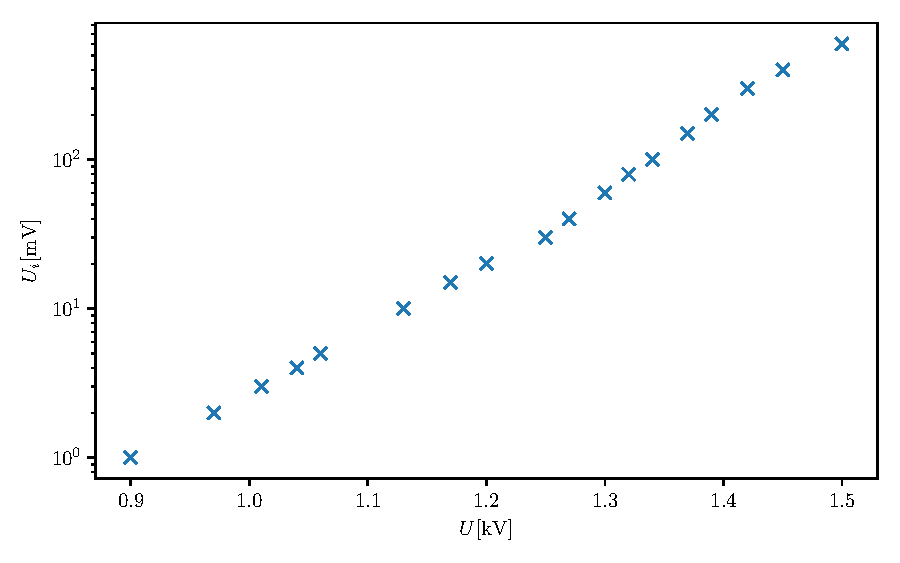
\includegraphics{u6.pdf}
        \caption{Závislost elektrického impulsu Geiger-Müllerova detektoru na přiloženém napětí}
        \label{fig:u6}
    \end{figure}

    \section*{Diskuse}

    Hodnoty ionizačního proudu poměrně výrazně kmitaly, nebylo proto snadné určit správnou hodnotu a tomu odpovídají chyby hodnot.
    Hodnoty vzdáleností $d$ byly považovány za přesné.

    Hodnota tekoucího proudu ionizační komorou bez elektrického napětí při vzdálenosti $d = \SI{2}{cm}$ v tabulce~\ref{tab:u2} je anomální, jedná se zřejmě o artefakt zapojení (alespoň podle asistenta praktika).
    Jak bylo již uvedeno výše, svodový proud byl i při vysokém napětí prakticky neměřitelný, neionizovaný vzduch vyplňující ionizační komoru je tedy velmi dobrý izolant.

    Spočítané hodnoty aktivit zářičů se významně liší od skutečných hodnot.
    To je zřejmě způsobeno tím, že $\alpha$ částice ztrácí energii i jiným mechanizmem, nežli jen ionizací.
    Poměr vypočítaných aktivit $\frac{A_{EA13}}{A_{EA14}} = \si{0,063}$ je však blízká poměru skutečných aktivit $\si{0,067}$.
    Rozdíl těchto poměrů lze vysvětlit tím, že částice $\alpha$ mají dráhu doletu o něco větší, než je $d = \SI{6}{cm}$ a tudíž částice vylétající ze zdroje směrem kolmým na elektrody nemusí ztratit všechnu energii v komoře.
    
    Z důvodu malé citlivosti osciloskopu nebylo možné proměřit celou voltampérovou charakteristiku Geiger-Müllerova detektoru.

    \section*{Závěr}

    Silnějším zářičem je zářič EA14.
    Změřené voltampérové charakteristiky odpovídají teoretickým předpovědím a byly náležitě popsány.
    Byly nalezené optimální podmínky pro měření s ionizační komorou, $U = \SI{500}{V}$, $d = \SI{6}{cm}$.
    Vypočtené aktivity zářičů výrazně podhodnocují skutečné aktivity, ale poměry aktivit vcelku odpovídají skutečnosti.

    \begin{thebibliography}{}

        \bibitem{pokyny}
        Pokyny k měření ``Studium plynových detektorů'', dostupné z\\ \url{https://physics.mff.cuni.cz/vyuka/zfp/_media/zadani/texty/txt_402.pdf}, 7.\,11.\,2019

    \end{thebibliography}

\end{document}